\section{Primo metodo (1984)}\logo{}
\subsection{Panoramica del metodo}\begin{frame}\frametitle{Panoramica del metodo}

Questo metodo\cite{1984} sviluppato nel 1984 e pubblicato su Chemosphere impiega una classica, lunga e  {\bf laboriosa purificazione} seguita da una  {\bf gascromatografia} ad alta risoluzione accoppiata a  {\bf spettrometria di massa a bassa risoluzione} in modalità \emph{selected ion monitoring}. 
\pause

La  {\bf ionizzazione ad ioni negativi} avviene ad opera di un plasma di ossigeno ed è  {\bf selettiva per le diossine} (i PCB ed altri interferenti hanno basse efficienze di ionizzazione).

Il picco a 176 Th è specifico delle 2:2 TCDD [Mitchum, Korfmacher, Moler, Stalling. 1982].\pause

La  {\bf quantificazione sfrutta l'aggiunta di uno standard interno interamente marcato $^{13}$C}. 

\begin{figure}{\centering{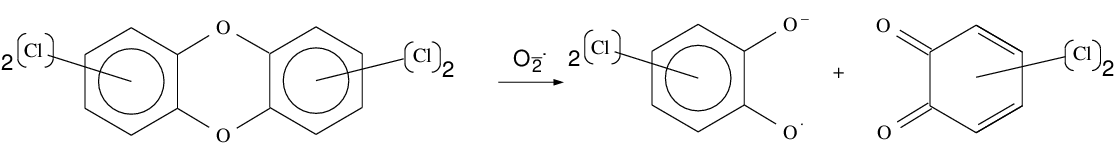
\includegraphics[width=1\textwidth]{img/diossineox.png}}}\end{figure}


\end{frame}\logo{
\includegraphics[width=0.1\paperwidth]{img/unipilogo.jpg}}

\subsection{Validità di HRGC-NIAPI-MS: analisi di soluzioni arricchite}\subsubsection{Campioni e pretrattamento}\begin{frame}\frametitle{Validità di HRGC-NIAPI-MS: analisi di soluzioni arricchite}\framesubtitle{Campioni e pretrattamento}

Per validare il metodo analitico sono stati analizzati campioni di  {\bf solventi arricchiti da altri laboratori ed analizzati tal quali}.\pause
\begin{description}
\item [{Campioni ricevuti da altri laboratori:}] 20 soluzioni in benzene di 60$\mu$L arricchite con varie concentrazioni di 2,3,7,8-TCDD. Alcune arricchite anche di altri pesticidi ed isomeri del TCDD;
\item [{Standard interno:}]  {\bf aggiunta di 2,3,7,8-TCDD-$^{13}$C come standard interno};
\item [{Estrazione, lavaggio e concentrazione:}] nessuna;

\end{description}



\end{frame}\subsubsection{Strumentazione di analisi}\begin{frame}\frametitle{Validità di HRGC-NIAPI-MS: analisi di soluzioni arricchite}\framesubtitle{Strumentazione di analisi}
\begin{description}

\item [{Analisi strumentale:}] HRGC-NIAPI-MS \begin{itemize}\pause
                                              \item  {\bf Gas cromatografia ad alta risoluzione operante isotermicamente} 
                                              \item {\bf Spettrometro di massa a bassa risoluzione in modalità selected ion monitoring}
                                              \begin{itemize}
                                               \item Sorgente  {\bf ionizzatore a pressione ambiente formante ioni negativi} utilizzando come gas di makeup azoto con 0.1\% di ossigeno (la ionizzazione avviene ad opera di \ce{O2-^.});
                                               \item Analizzatore  {\bf  quadrupolo che filtra} a rotazione tre m/z (Th) diversi: 176, 178 e 182;
                                              \end{itemize}
                                             \end{itemize} 

\end{description}

\end{frame}
\logo{}
\subsubsection{Criteri di conferma}\begin{frame}\frametitle{Validità di HRGC-NIAPI-MS: analisi di soluzioni arricchite}\framesubtitle{Criteri di conferma}


Criteri di conferma:\pause

\begin{itemize}
                                              \item l'area a 176 Th deve essere almeno 3 volte la sua deviazione standard;
                                              \item l'area a 178 Th deve essere almeno 3 volte la sua deviazione standard;
                                              \item il rapporto tra aree a 178 Th e 176 Th deve essere in accordo con la distribuzione isotopica al 99\% di confidenza;
                                              \item il tempo di  ritenzione del picco a 176 Th deve essere compreso nella finestra di ritenzione del picco a 182 Th (il picco a 182 Th appartiene solo al 2,3,7,8-TCDD-$^{13}$C perché solo questo isomero è stato aggiunto).
                                             \end{itemize} 


\end{frame}\logo{
\includegraphics[width=0.1\paperwidth]{img/unipilogo.jpg}}
\subsubsection{Risultati}\begin{frame}\frametitle{Validità di HRGC-NIAPI-MS: analisi di soluzioni arricchite}\framesubtitle{Risultati}\pause
\begin{description}

\item [{Analisi delle soluzioni senza aggiunta di interferenti:}] LOD $\approx$ 4ppt in un ipotetico campione di 10g estratto con recupero del 100\% ossia 40pg forniti nella soluzione. I risultati mostrano una certa eteroschedasticità ed una deviazione verso valori più positivi.
\end{description}
\begin{figure}{\centering{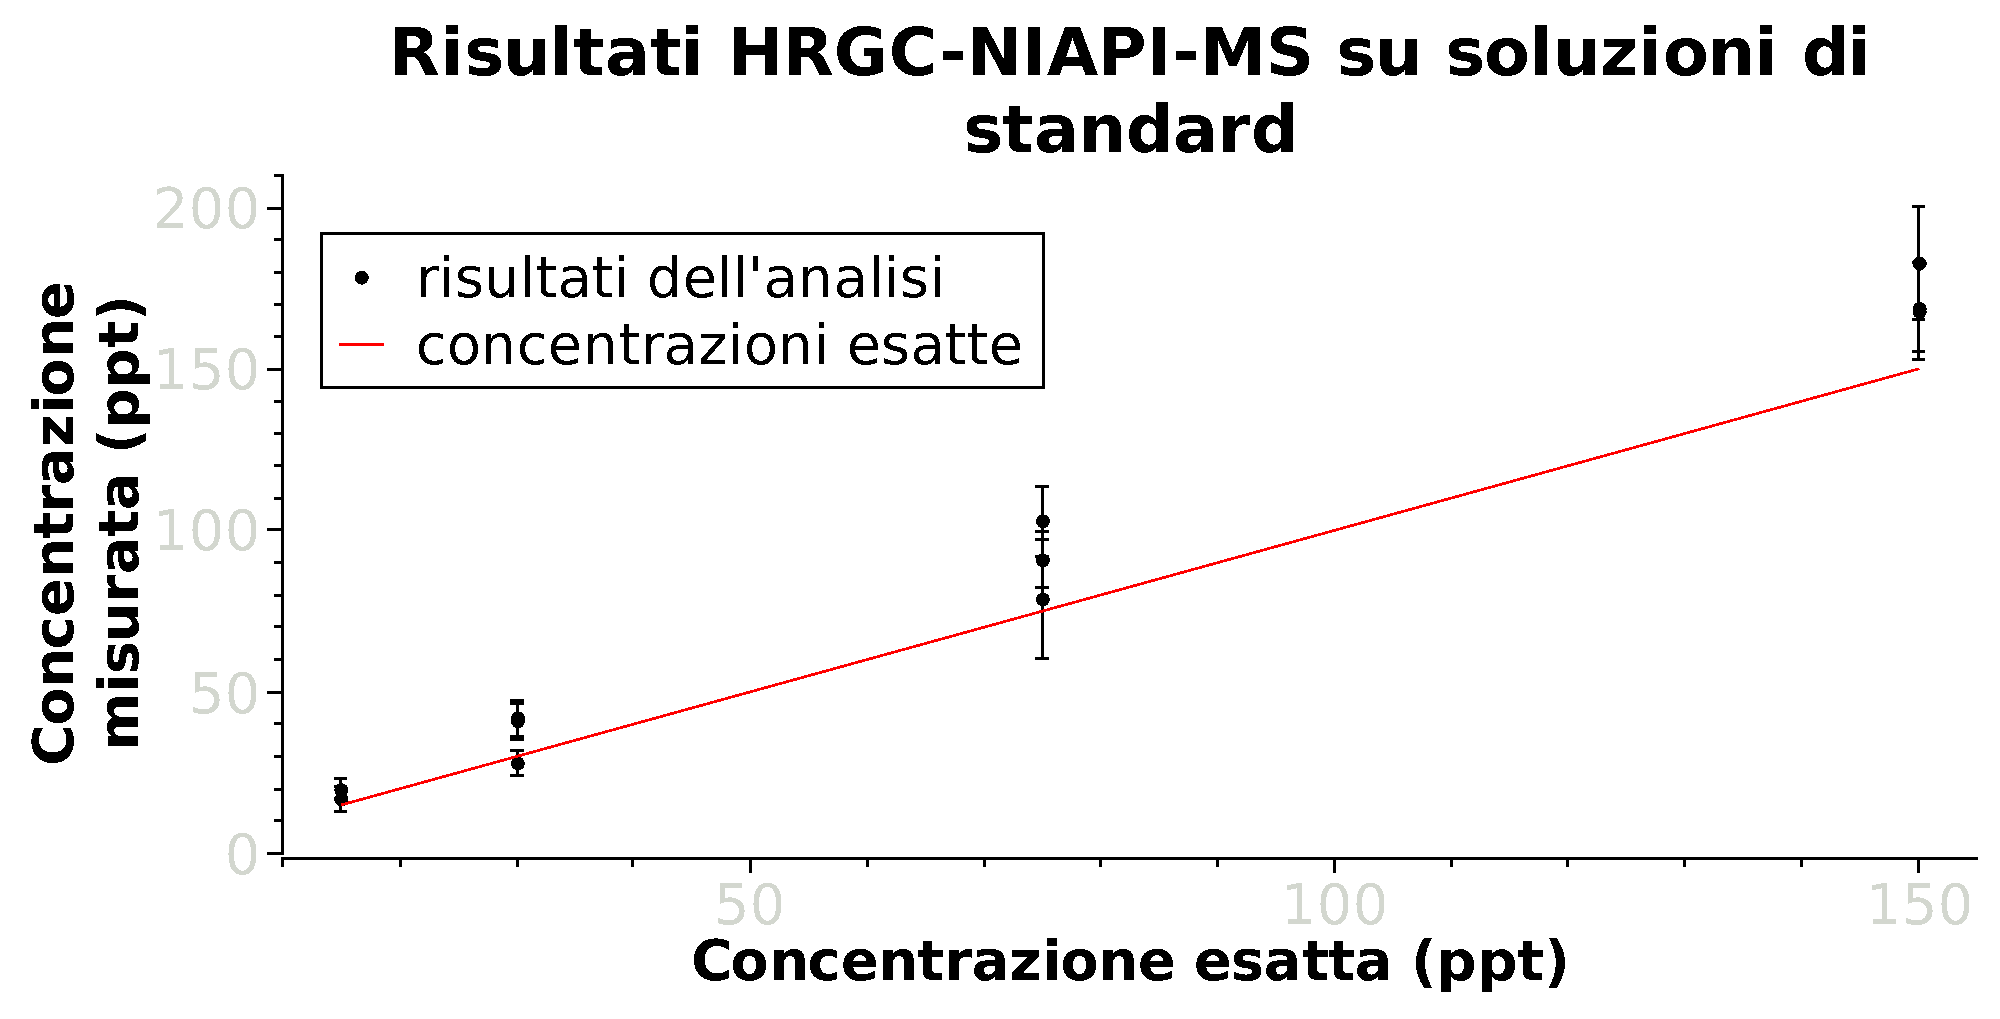
\includegraphics[width=0.7\textwidth]{img/analisisoluzstd.pdf}}}\end{figure}


\end{frame}


\begin{frame}\frametitle{Validità di HRGC-NIAPI-MS: analisi di soluzioni arricchite}\framesubtitle{Risultati}
\begin{description}

\item [{Analisi delle soluzioni con aggiunta di interferenti:}]\pause nel caso di  {\bf aggiunta di altri interferenti} classici come pp'DDE, Aroclor 1254 (una classe di   aromatici clorurati) o clordano (alifatico clorurato)  {\bf i risultati rimangono accettabili tranne in un caso in cui si rileva un valore molto minore} della quantità aggiunta di TCDD. Questo è facilmente motivabile con un  {\bf esaurimento del plasma di ossigeno} ad opera degli interferenti. Comunque ricordiamo che questi  {\bf risultati sono ottenuti in assenza di lavaggio}, processo che avrebbe rimosso gli interferenti.

\end{description}





\end{frame}


\diapo{Valutazione del recupero dello standard interno}

Il recupero dello standard interno 2,3,7,8-TCDD-$^{14}$C da una matrice di pesce gatto \pause è stato trattato in un articolo a cui non si può sperar di avere accesso, i pochi dati riportati sono:
 \begin{itemize}
  \item l'essiccazione in {\bf flusso di azoto} quando utilizzata a temperature maggiori di 50°C comporta  {\bf grandi perdite};
  \item  {\bf migliore} è il metodo di  {\bf centrifugazione a vuoto};
  \item utilizzando il secondo sistema di concentrazione si sono ottenuti  {\bf recuperi del 40\% }(misurando campioni arricchiti a 200ppt).
 \end{itemize}


\end{frame}
\logo{}
\subsection{Valutazione dell'estrazione: analisi di campioni di suolo}\subsubsection{Arricchimento, pretrattamento, estrazione e lavaggio}\begin{frame}\frametitle{Valutazione dell'estrazione: analisi di campioni di suolo}\framesubtitle{Arricchimento, pretrattamento, estrazione e lavaggio}
{\scriptsize
\begin{itemize}
 \item  {\bf 10g di suolo in pallone arricchiti con 100ppt di 2,3,7,8-TCDD-$^{13}$C};\pause
 \item  aggiunti 60mL di  {\bf potassa alcolica} (KOH 45\%/EtOH = 2/1) e scaldato a riflusso per 2.5h;
 \item filtrazione su  {\bf filtro in Teflon};
 \item  {\bf estrazione} in imbuto separatore con 4 aliquote da 50mL di  {\bf n-esano};
 \item  {\bf lavaggio con KOH} 1M, 4  {\bf lavaggi con acido solforico concentrato}, lavaggio con acqua e neutralizzazione con \ce{Na2CO3};
 \item la fase organica viene passata in una  {\bf colonna} contenente (dalla cima al fondo): \ce{Na2CO3}, \ce{Na2SO4}, 50\% allumina acida + 50\% allumina basica;
 \item il risultante estratto viene ridotto di volume, viene aggiunto benzene, viene versato in una provetta da centrifuga e portato a secco con  {\bf centrifugazione a vuoto a temperatura ambiente};
 \item ridissoluzione in benzene, iniezione in  {\bf colonna HPLC di silice} con esano come eluente e raccolta della frazione contenente il TCDD;
 \item essiccamento con centrifugazione a vuoto a temperatura ambiente;
 \item ridissoluzione in benzene, iniezione in  {\bf 2 colonne HPLC a fase inversa in serie} con acetonitrile come eluente e raccolta della frazione contenente il TCDD;
 \item essiccamento con centrifugazione a vuoto a temperatura ambiente;
 \item ridissoluzione in 30$\mu$L di benzene ed  {\bf iniezione in due aliquote} nell'apparato di analisi HRGC-NIAPI-MS. 
\end{itemize}}
\end{frame}\logo{
\includegraphics[width=0.1\paperwidth]{img/unipilogo.jpg}}
\subsubsection{Risultati}\begin{frame}\frametitle{Valutazione dell'estrazione: analisi di campioni di suolo}\framesubtitle{Risultati}\pause
Le analisi di campioni di  {\bf terreno argilloso arricchiti con solo 2,3,7,8-TCDD} all'interno di uno studio interlaboratorio danno risultati in buono accordo con i  {\bf valori di fortificazione dei campioni}. Si ottiene un LOD $\approx$ 5ppt ossia 50pg di 2,3,7,8-TCDD nel campione. Non viene riportato un confronto coi risultati degli altri laboratori.

\begin{figure}{\centering{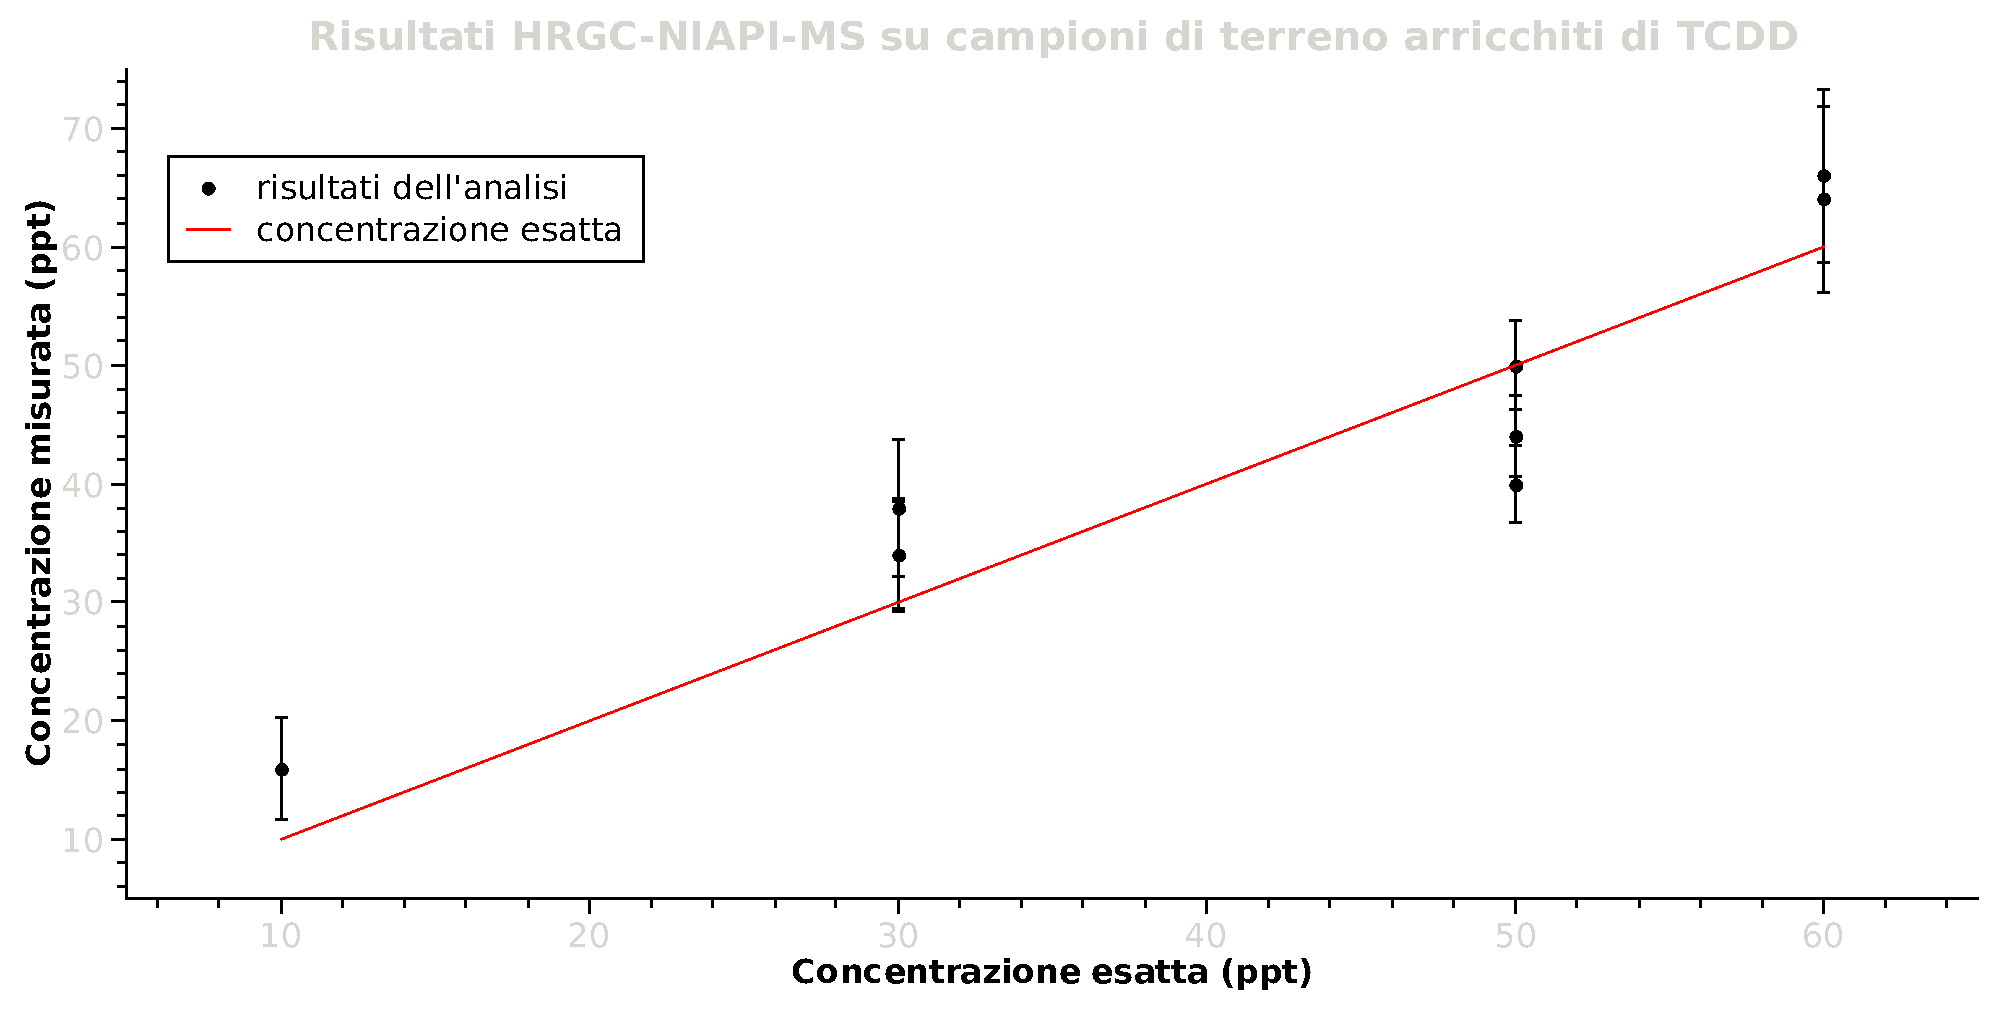
\includegraphics[width=0.8\textwidth]{img/analisiterr.pdf}}}\end{figure}



\end{frame}

\logo{}


\diapo{Valutazione della separazione: suolo con interferenti}\pause

Nelle analisi di campioni di terreno fortificati anche  {\bf con interferenti} come altri isomeri del 2,3,7,8-TCDD, Aroclor 1254, Aroclor 1260 e pp'DDE  {\bf non si riscontrano grosse differenze} rispetto al caso precedente.
\begin{figure}{\centering{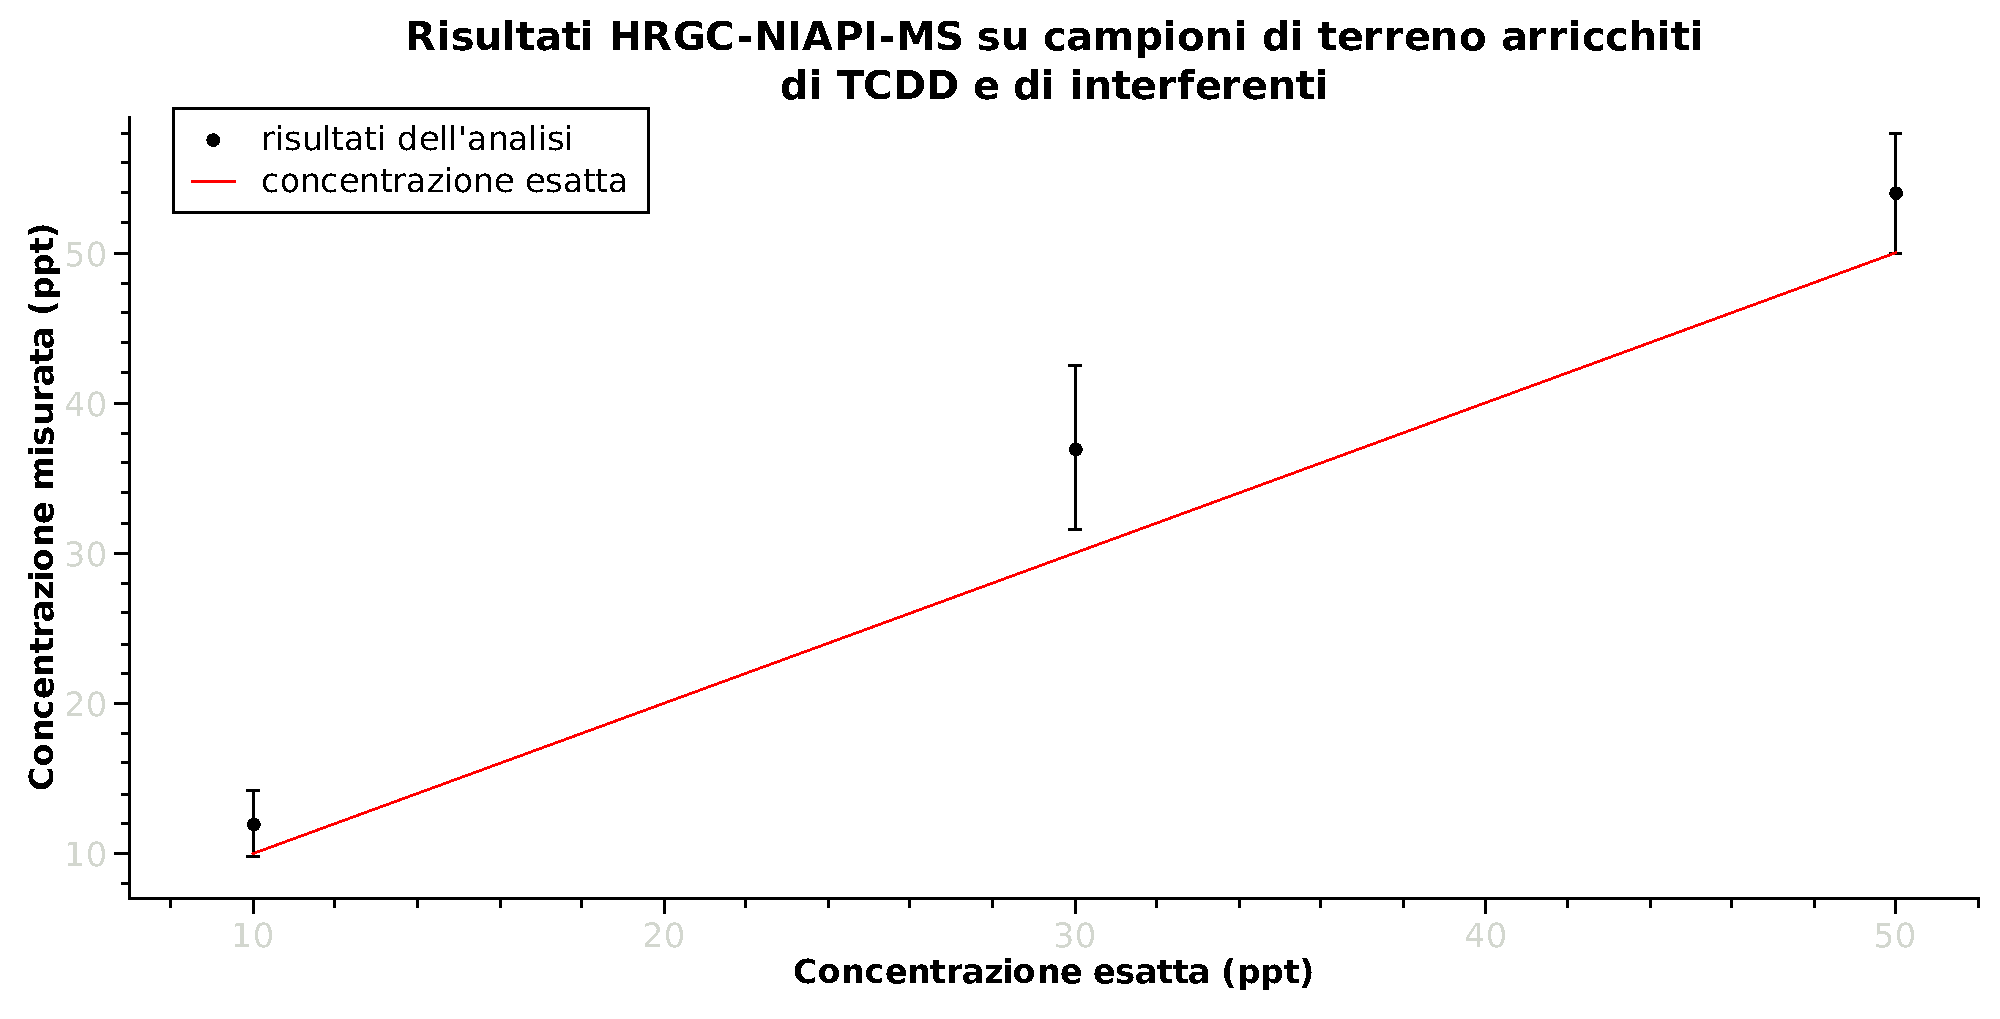
\includegraphics[width=0.9\textwidth]{img/analisiterrinterf.pdf}}}\end{figure}


\end {frame}\logo{
\includegraphics[width=0.1\paperwidth]{img/unipilogo.jpg}}

\subsection{Conclusioni}\begin{frame}\frametitle{Conclusioni}
Sono state valutati i seguenti parametri:\pause
  \begin{itemize}
\item[\checkmark] esattezza rispetto ai valori di fortificazione incogniti,
 \item[\checkmark] precisione,\pause
 \item[\checkmark] recupero di uno standard interno,\pause
 \item[\checkmark] campo di applicazione ad altre matrici (sono state testate 5 matrici),\pause
 \item[\checkmark] selettività in presenza di isomeri ed interferenti,\pause
 \item[\checkmark] limite di rivelabilità,
 \item[\checkmark] valutazione del bianco,
\end{itemize}
\end{frame}
\begin{frame}\frametitle{Conclusioni}
{\bf Non} sono state valutati i seguenti parametri:\pause
  \begin{itemize}
 \item[$\times$] robustezza,
 \item[$\times$] ottimizzazione,
 \item[$\times$] riproducibilità,
 \item[$\times$] incertezza,
 \item[$\times$] valutazione dell'effetto matrice col metodo delle aggiunte,\pause
 \item[$\times$] range dinamico e lineare,\pause
 \item[$\times$] confronto coi risultati interlaboratorio (presentati in un documento non ottenibile),\pause
 \item[$\times$] parametri di qualità e criteri di accettazione,
 \item[$\times$] campo di applicazione ad altri analiti.
\end{itemize}
\end{frame}






